\item[12]  Here is  a list  of  four propositional  forms  and two  circuits. This  list
  contains three pairs of logically equivalent entries (we will say a circuit is equivalent
  to a propositional form  if the propositional form describes the  value of the circuit's
  output for all possible combinations of input values). For instance, maybe $A \equiv B$,
  $C \equiv D$, and $E  \equiv F$). First determine  the three pairs, and then
  prove for each pair that one element of the pair is logically equivalent to the other
  one.
  \begin{enumerate}[(A)]
  \item $(\lnot a \land b) \iff \lnot(c \lor d)$.
  \item $(\lnot a \lor b)\land(\lnot a \lor c)\land(\lnot a \lor \lnot d)$
  \item $(a \land b \land c)\lor \lnot(b \land c \land d)$.
  \item $a \implies (b \land c \land \lnot d)$. 
  \item \leavevmode\lower45pt\hbox{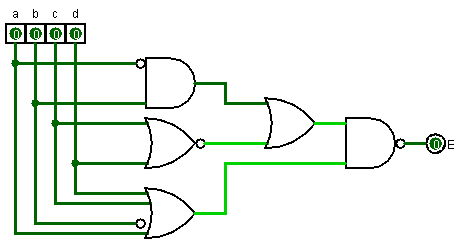
\includegraphics[scale=0.75]{hw1-q2e.png}}
  \item \leavevmode\lower45pt\hbox{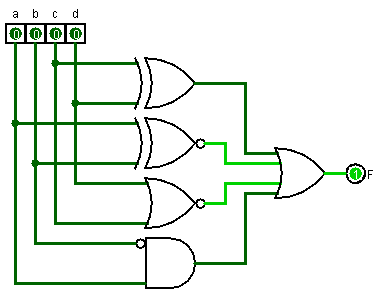
\includegraphics[scale=0.75]{hw1-q2f.png}}
  \end{enumerate}

  You are  allowed to use truth  tables to figure  out the equivalences; however  at least
  two of your proofs must use a  sequence of known logical equivalences (see Epp table
  2.1.1, or Dave's formula sheet; you can also assume that $x \implies y \equiv \;
  {\lnot x  \vee y}$ and that  $x \oplus y  \equiv (x \lor  y)\, \land \sim\! (x  \land y)
  \equiv (\lnot  x \land y)  \lor (x \land  \lnot y)$. The third proof can use either a
  sequence of known logical equivalences, or a truth table.

  Hint: you might want to translate the  circuits into formulas that mirror exactly as the
  circuit is implemented, before using any logical equivalence rules.
  \newpage
\begin{enumerate}
\item \LARGE\underline{~~~~~~~~~}$\equiv$\underline{~~~~~~~~~~}\\

\begin{tabular}{rcl|l}
~~~~~~expression 1 & & expression 2~~~~~~ & reason \\
\hline
& $\equiv$ & & ~~~~~~~~~~~~~~~~~~~~~~~\\
\hline
& $\equiv$ & & ~~~~~~~~~~~~~~~~~~~~~~~\\
\hline
& $\equiv$ & & ~~~~~~~~~~~~~~~~~~~~~~~\\
\hline
& $\equiv$ & & ~~~~~~~~~~~~~~~~~~~~~~~\\
\hline
& $\equiv$ & & ~~~~~~~~~~~~~~~~~~~~~~~\\
\hline
& $\equiv$ & & ~~~~~~~~~~~~~~~~~~~~~~~\\
\hline
& $\equiv$ & & ~~~~~~~~~~~~~~~~~~~~~~~\\
\hline
& $\equiv$ & & ~~~~~~~~~~~~~~~~~~~~~~~\\
\hline
& $\equiv$ & & ~~~~~~~~~~~~~~~~~~~~~~~\\
\hline
& $\equiv$ & & ~~~~~~~~~~~~~~~~~~~~~~~\\
\hline
& $\equiv$ & & ~~~~~~~~~~~~~~~~~~~~~~~\\
\hline
& $\equiv$ & & ~~~~~~~~~~~~~~~~~~~~~~~\\
\hline
& $\equiv$ & & ~~~~~~~~~~~~~~~~~~~~~~~\\
\hline
& $\equiv$ & & ~~~~~~~~~~~~~~~~~~~~~~~\\
\hline
& $\equiv$ & & ~~~~~~~~~~~~~~~~~~~~~~~\\
\hline
& $\equiv$ & & ~~~~~~~~~~~~~~~~~~~~~~~\\
\hline
& $\equiv$ & & ~~~~~~~~~~~~~~~~~~~~~~~\\
\hline
& $\equiv$ & & ~~~~~~~~~~~~~~~~~~~~~~~\\
\hline
& $\equiv$ & & ~~~~~~~~~~~~~~~~~~~~~~~\\
\hline
& $\equiv$ & & ~~~~~~~~~~~~~~~~~~~~~~~\\
\hline
\end{tabular}\\
\large
\newpage
\item \LARGE\underline{~~~~~~~~~}$\equiv$\underline{~~~~~~~~~~}\\

\begin{tabular}{rcl|l}
~~~~~~expression 1 & & expression 2~~~~~~ & reason \\
\hline
& $\equiv$ & & ~~~~~~~~~~~~~~~~~~~~~~~\\
\hline
& $\equiv$ & & ~~~~~~~~~~~~~~~~~~~~~~~\\
\hline
& $\equiv$ & & ~~~~~~~~~~~~~~~~~~~~~~~\\
\hline
& $\equiv$ & & ~~~~~~~~~~~~~~~~~~~~~~~\\
\hline
& $\equiv$ & & ~~~~~~~~~~~~~~~~~~~~~~~\\
\hline
& $\equiv$ & & ~~~~~~~~~~~~~~~~~~~~~~~\\
\hline
& $\equiv$ & & ~~~~~~~~~~~~~~~~~~~~~~~\\
\hline
& $\equiv$ & & ~~~~~~~~~~~~~~~~~~~~~~~\\
\hline
& $\equiv$ & & ~~~~~~~~~~~~~~~~~~~~~~~\\
\hline
& $\equiv$ & & ~~~~~~~~~~~~~~~~~~~~~~~\\
\hline
& $\equiv$ & & ~~~~~~~~~~~~~~~~~~~~~~~\\
\hline
& $\equiv$ & & ~~~~~~~~~~~~~~~~~~~~~~~\\
\hline
& $\equiv$ & & ~~~~~~~~~~~~~~~~~~~~~~~\\
\hline
& $\equiv$ & & ~~~~~~~~~~~~~~~~~~~~~~~\\
\hline
& $\equiv$ & & ~~~~~~~~~~~~~~~~~~~~~~~\\
\hline
& $\equiv$ & & ~~~~~~~~~~~~~~~~~~~~~~~\\
\hline
& $\equiv$ & & ~~~~~~~~~~~~~~~~~~~~~~~\\
\hline
& $\equiv$ & & ~~~~~~~~~~~~~~~~~~~~~~~\\
\hline
& $\equiv$ & & ~~~~~~~~~~~~~~~~~~~~~~~\\
\hline
& $\equiv$ & & ~~~~~~~~~~~~~~~~~~~~~~~\\
\hline
\end{tabular}
\large
\newpage
\item \LARGE\underline{~~~~~~~~~}$\equiv$\underline{~~~~~~~~~~}\\
\newpage
\end{enumerate}